% \VignetteEngine{knitr::knitr}
% \VignetteIndexEntry{ccrepe}

\documentclass{article}\usepackage[]{graphicx}\usepackage[usenames,dvipsnames]{color}
% maxwidth is the original width if it is less than linewidth
% otherwise use linewidth (to make sure the graphics do not exceed the margin)
\makeatletter
\def\maxwidth{ %
  \ifdim\Gin@nat@width>\linewidth
    \linewidth
  \else
    \Gin@nat@width
  \fi
}
\makeatother

\definecolor{fgcolor}{rgb}{0.251, 0.251, 0.251}
\newcommand{\hlnum}[1]{\textcolor[rgb]{0.816,0.125,0.439}{#1}}%
\newcommand{\hlstr}[1]{\textcolor[rgb]{0.251,0.627,0.251}{#1}}%
\newcommand{\hlcom}[1]{\textcolor[rgb]{0.502,0.502,0.502}{\textit{#1}}}%
\newcommand{\hlopt}[1]{\textcolor[rgb]{0,0,0}{#1}}%
\newcommand{\hlstd}[1]{\textcolor[rgb]{0.251,0.251,0.251}{#1}}%
\newcommand{\hlkwa}[1]{\textcolor[rgb]{0.125,0.125,0.941}{#1}}%
\newcommand{\hlkwb}[1]{\textcolor[rgb]{0,0,0}{#1}}%
\newcommand{\hlkwc}[1]{\textcolor[rgb]{0.251,0.251,0.251}{#1}}%
\newcommand{\hlkwd}[1]{\textcolor[rgb]{0.878,0.439,0.125}{#1}}%
\let\hlipl\hlkwb

\newenvironment{knitrout}{}{} % an empty environment to be redefined in TeX
\usepackage{alltt}

%% -------------------------
%% Pre-amble:
%% -------------------------

\usepackage{float}
\usepackage[nonamebreak,square]{natbib}
\usepackage{amsmath}

\RequirePackage[]{/home/jakobpp/anaconda3/envs/micInt/lib/R/library/BiocStyle/resources/tex/Bioconductor}




\title{CCREPE: Compositionality Corrected by PErmutation and REnormalization}
\author{Emma Schwager, George Weingart, Craig Bielski, Curtis Huttenhower}

%% -------------------------
%% End pre-amble
%% -------------------------
\IfFileExists{upquote.sty}{\usepackage{upquote}}{}
\begin{document}

\maketitle

\tableofcontents

\section{Introduction}

\Biocpkg{ccrepe} is a package for analysis of sparse compositional data.  Specifically, it determines the significance of association between features in a composition, using any similarity measure (e.g. Pearson correlation, Spearman correlation, etc.)  The CCREPE methodology stands for Compositionality Corrected by Renormalization and Permutation, as detailed below.  The package also provides a novel similarity measure, the N-dimensional checkerboard score (NC-score), particularly appropriate to compositions derived from microbial community sequencing data.  This results in p-values and false discovery rate q-values corrected for the effects of compositionality.  The package contains two functions \Rfunction{ccrepe} and \Rfunction{nc.score} and is maintained by the Huttenhower lab (\email{ccrepe-users@googlegroups.com}).

%---------------------------------------------------------
\section{ccrepe} 
%---------------------------------------------------------

\Rfunction{ccrepe} is the main package function.  It calculates compositionality-corrected p-values and q-values for a user-selected similarity measure, operating on either one or two input matrices.  If given one matrix, all features (columns) in the matrix are compared to each other using the selected similarity measure.  If given two matrices, each feature in the first are compared against all features in the second.

\subsection{General functionality}

Compositional data induces spurious correlations between features due to the nonindependence of values that must sum to a fixed total.  CCREPE abrogates this when determining the significance of a similarity measure for each feature pair using two main steps, permutation/renormalization and bootstrapping.  First, given two features to compare, CCREPE generates a null distribution of the similarity expected just due to compositionality by iteratively permuting one feature, renormalizing all samples in the composition to their previous sum, and computing the resulting similarity measures.  Second, CCREPE bootstraps over sample subsets in order to assess confidence in the "true" similarity measure.  Finally, the two resulting distributions are compared using a pooled-variance Z-test to give a compositionality-corrected p-value.  False discovery rate q-values are additionally calculated using the Benjamin-Hochberg-Yekutieli procedure.  For greater detail, see \citet{faust2012microbial} and \citet{schwager2012unpublished}.\\

CCREPE employs several filtering steps before the data are processed.  It removes any missing subjects using \Rcode{na.omit}: in the two dataset case, any subjects missing in \emph{either} dataset will be removed.  Any subjects or features which are all zero are removed as well: an all-zero subject cannot be normalized (its sum is 0) and an all-zero feature has standard deviation 0 (in addition to being uninteresting biologically).

\subsection{Arguments}

\begin{description}
\setlength{\itemsep}{1em}

\item[\Rcode{x}]
First \Rclass{dataframe} or \Rclass{matrix} containing relative abundances.  Columns are features, rows are samples.  Rows should therefore sum to a constant.  Row names are used for identification if present.

\item[\Rcode{y}]
Second \Rclass{dataframe} or \Rclass{matrix} (optional) containing relative abundances.  Columns are features, rows are samples.  Rows should therefore sum to a constant.  If both \Rcode{x} and \Rcode{y} are specified, they will be merged by row names.  If no row names are specified for either or both datasets,   the default is to merge by row number.

\item[\Rcode{sim.score}]
Similarity measure, such as \Rfunction{cor} or \Rfunction{nc.score}.  This can be either an existing R function or user-defined.  If the latter, certain properties should be satisfied as detailed below (also see examples).  The default similarity measure is the Pearson correlation.

A user-defined similarity measure should mimic the interface of \Rfunction{cor}:
\begin{enumerate}
\item Take either two \Rclass{vector} inputs one \Rclass{matrix} or \Rclass{dataframe} input.

\item In the case of two inputs, return a single number.

\item In the case of one input, return a matrix in which the (\Rcode{i},\Rcode{j})th entry is the similarity score for column \Rcode{i} and column \Rcode{j} in the original matrix.

\item The resulting matrix (in the case of one input) must be symmetric.

\item The inputs must be named \Rcode{x} and \Rcode{y}.
\end{enumerate}

\item[\Rcode{sim.score.args}]
An optional list of arguments for the measurement function.  When given, they are passed to the \Rcode{sim.score} function directly.  For example, in the case of \Rcode{cor}, the following would be acceptable:

\begin{knitrout}
\definecolor{shadecolor}{rgb}{0.941, 0.941, 0.941}\color{fgcolor}\begin{kframe}
\begin{alltt}
\hlstd{sim.score.args} \hlkwb{=} \hlkwd{list}\hlstd{(}\hlkwc{method}\hlstd{=}\hlstr{"spearman"}\hlstd{,} \hlkwc{use}\hlstd{=}\hlstr{"complete.obs"}\hlstd{)}
\end{alltt}
\end{kframe}
\end{knitrout}

\item[\Rcode{min.subj}]
Minimum number (count) of samples that must be non-missing in order to apply the similarity measure.  This is to ensure that there are sufficient samples to perform a bootstrap (default: 20).

\item[\Rcode{iterations}]
The number of iterations for both bootstrap and permutation calculations (default: 1000).

\item[\Rcode{subset.cols.x}]
A vector of column indices from x to indicate which features to compare

\item[\Rcode{subset.cols.y}]
A vector of column indices from y to indicate which features to compare

\item[\Rcode{errthresh}]
If feature has number of zeros greater than   $\ errthresh^{1/n} $  , that feature is excluded     

\item[\Rcode{verbose}]
If \Rcode{TRUE}, print periodic progress of the algorithm through the dataset(s), as well as including more detailed debugging output.  (default: \Rcode{FALSE}).

\item[\Rcode{iterations.gap}]
If \Rcode{verbose=TRUE}, the number of iterations between issuing status messages (default: 100).

\item[\Rcode{distributions}]
Optional output file for detailed log (if given) of all intermediate permutation and renormalization distributions.

\item[\Rcode{compare.within.x}]
  A boolean value indicating whether to do comparisons given by taking all subsets of size 2 from \Rcode{subset.cols.x} or to do comparisons given by taking all possible combinations of \Rcode{subset.cols.x} and \Rcode{subset.cols.y}.  If \Rcode{TRUE} but \Rcode{subset.cols.y=NA}, returns all comparisons involving any features in \Rcode{subset.cols.x}.  This argument is only used when \Rcode{y=NA}.
  
\item[\Rcode{concurrent.output}]
    Optional output file to which each comparison will be written as it is calculated.
    
\item[\Rcode{make.output.table}]
      A boolean value indicating whether to include table-formatted output.

\end{description}

\subsection{Output}

\Rcode{ccrepe} returns a \Rclass{list} containing both the calculation results and the parameters used:

\begin{description}
\setlength{\itemsep}{1em}

\item[\Rcode{sim.score}]
\Rclass{matrix} of simliarity scores for all requested comparisons.  The (\Rcode{i},\Rcode{j})th element corresponds to the similarity score of column \Rcode{i} (or the \Rcode{i}th column of \Rcode{subset.cols.1}) and column \Rcode{j} (or the \Rcode{j}th column of \Rcode{subset.cols.1}) in one dataset, or to the similarity score of column \Rcode{i} (or the \Rcode{i}th column of \Rcode{subset.cols.1}) in dataset \Rcode{x} and column \Rcode{j} (or the \Rcode{j}th column of \Rcode{subset.cols.2}) in dataset \Rcode{y} in the case of two datasets.

\item[\Rcode{p.values}]
\Rclass{matrix} of the corrected p-values for all requested comparisons.  The (\Rcode{i},\Rcode{j})th element corresponds to the p-value of the (\Rcode{i},\Rcode{j})th element of \Rcode{sim.score}.

\item[\Rcode{q.values}]
\Rclass{matrix} of the Benjamini-Hochberg-Yekutieli corrected p-values.  The (\Rcode{i},\Rcode{j})th element corresponds to the p-value of the (\Rcode{i},\Rcode{j})th element of \Rcode{sim.score}.

\item[\Rcode{z.stat}]
  \Rclass{matrix} of the z-statistics used in generating the p-values for all requested comparisons.  The (\Rcode{i},\Rcode{j})th element corresponds to the z-statistic generating the (\Rcode{i},\Rcode{j})th element of \Rcode{p.values}.

\end{description}

\subsection{Usage}	

\begin{knitrout}
\definecolor{shadecolor}{rgb}{0.941, 0.941, 0.941}\color{fgcolor}\begin{kframe}
\begin{alltt}
\hlkwd{ccrepe}\hlstd{(}
 \hlkwc{x} \hlstd{=} \hlnum{NA}\hlstd{,}
 \hlkwc{y} \hlstd{=} \hlnum{NA}\hlstd{,}
 \hlkwc{sim.score} \hlstd{= cor,}
 \hlkwc{sim.score.args} \hlstd{=} \hlkwd{list}\hlstd{(),}
 \hlkwc{min.subj} \hlstd{=} \hlnum{20}\hlstd{,}
 \hlkwc{iterations} \hlstd{=} \hlnum{1000}\hlstd{,}
 \hlkwc{subset.cols.x} \hlstd{=} \hlkwa{NULL}\hlstd{,}
 \hlkwc{subset.cols.y} \hlstd{=} \hlkwa{NULL}\hlstd{,}
 \hlkwc{errthresh}  \hlstd{=} \hlnum{1e-04}\hlstd{,}
 \hlkwc{verbose} \hlstd{=} \hlnum{FALSE}\hlstd{,}
 \hlkwc{iterations.gap} \hlstd{=} \hlnum{100}\hlstd{,}
 \hlkwc{distributions} \hlstd{=} \hlnum{NA}\hlstd{,}
 \hlkwc{compare.within.x} \hlstd{=} \hlnum{TRUE}\hlstd{,}
 \hlkwc{concurrent.output} \hlstd{=} \hlnum{NA}\hlstd{,}
 \hlkwc{make.output.table} \hlstd{=} \hlnum{FALSE}\hlstd{)}
\end{alltt}
\end{kframe}
\end{knitrout}

\subsection{Example 1}

An example of how to use \Rfunction{ccrepe} with one dataset.

\begin{knitrout}
\definecolor{shadecolor}{rgb}{0.941, 0.941, 0.941}\color{fgcolor}\begin{kframe}
\begin{alltt}
\hlstd{data} \hlkwb{<-} \hlkwd{matrix}\hlstd{(}\hlkwd{rlnorm}\hlstd{(}\hlnum{40}\hlstd{,}\hlkwc{meanlog}\hlstd{=}\hlnum{0}\hlstd{,}\hlkwc{sdlog}\hlstd{=}\hlnum{1}\hlstd{),}\hlkwc{nrow}\hlstd{=}\hlnum{10}\hlstd{,}\hlkwc{ncol}\hlstd{=}\hlnum{4}\hlstd{)}
\hlstd{data[,}\hlnum{1}\hlstd{]} \hlkwb{=} \hlnum{2}\hlopt{*}\hlstd{data[,}\hlnum{2}\hlstd{]} \hlopt{+} \hlkwd{rnorm}\hlstd{(}\hlnum{10}\hlstd{,}\hlnum{0}\hlstd{,}\hlnum{0.01}\hlstd{)}
\hlstd{data.rowsum} \hlkwb{<-} \hlkwd{apply}\hlstd{(data,}\hlnum{1}\hlstd{,sum)}
\hlstd{data.norm} \hlkwb{<-} \hlstd{data}\hlopt{/}\hlstd{data.rowsum}
\hlkwd{apply}\hlstd{(data.norm,}\hlnum{1}\hlstd{,sum)}  \hlcom{# The rows sum to 1, so the data are normalized}
\end{alltt}
\begin{verbatim}
##  [1] 1 1 1 1 1 1 1 1 1 1
\end{verbatim}
\begin{alltt}
\hlstd{test.input} \hlkwb{<-} \hlstd{data.norm}

\hlkwd{dimnames}\hlstd{(test.input)} \hlkwb{<-} \hlkwd{list}\hlstd{(}\hlkwd{c}\hlstd{(}
 \hlstr{"Sample 1"}\hlstd{,} \hlstr{"Sample 2"}\hlstd{,}\hlstr{"Sample 3"}\hlstd{,}\hlstr{"Sample 4"}\hlstd{,}\hlstr{"Sample 5"}\hlstd{,}
 \hlstr{"Sample 6"}\hlstd{,}\hlstr{"Sample 7"}\hlstd{,}\hlstr{"Sample 8"}\hlstd{,}\hlstr{"Sample 9"}\hlstd{,}\hlstr{"Sample 10"}\hlstd{),}
 \hlkwd{c}\hlstd{(}\hlstr{"Feature 1"}\hlstd{,} \hlstr{"Feature 2"}\hlstd{,} \hlstr{"Feature 3"}\hlstd{,}\hlstr{"Feature 4"}\hlstd{))}

\hlstd{test.output} \hlkwb{<-} \hlkwd{ccrepe}\hlstd{(}\hlkwc{x}\hlstd{=test.input,} \hlkwc{iterations}\hlstd{=}\hlnum{20}\hlstd{,} \hlkwc{min.subj}\hlstd{=}\hlnum{10}\hlstd{)}
\end{alltt}
\end{kframe}
\end{knitrout}
\begin{knitrout}
\definecolor{shadecolor}{rgb}{0.941, 0.941, 0.941}\color{fgcolor}\begin{kframe}
\begin{alltt}
\hlkwd{par}\hlstd{(}\hlkwc{mfrow}\hlstd{=}\hlkwd{c}\hlstd{(}\hlnum{1}\hlstd{,}\hlnum{2}\hlstd{))}
\hlkwd{plot}\hlstd{(data[,}\hlnum{1}\hlstd{],data[,}\hlnum{2}\hlstd{],}\hlkwc{xlab}\hlstd{=}\hlstr{"Feature 1"}\hlstd{,}\hlkwc{ylab}\hlstd{=}\hlstr{"Feature 2"}\hlstd{,}\hlkwc{main}\hlstd{=}\hlstr{"Non-normalized"}\hlstd{)}
\hlkwd{plot}\hlstd{(data.norm[,}\hlnum{1}\hlstd{],data.norm[,}\hlnum{2}\hlstd{],}\hlkwc{xlab}\hlstd{=}\hlstr{"Feature 1"}\hlstd{,}\hlkwc{ylab}\hlstd{=}\hlstr{"Feature 2"}\hlstd{,}
     \hlkwc{main}\hlstd{=}\hlstr{"Normalized"}\hlstd{)}
\end{alltt}
\end{kframe}\begin{figure}[H]
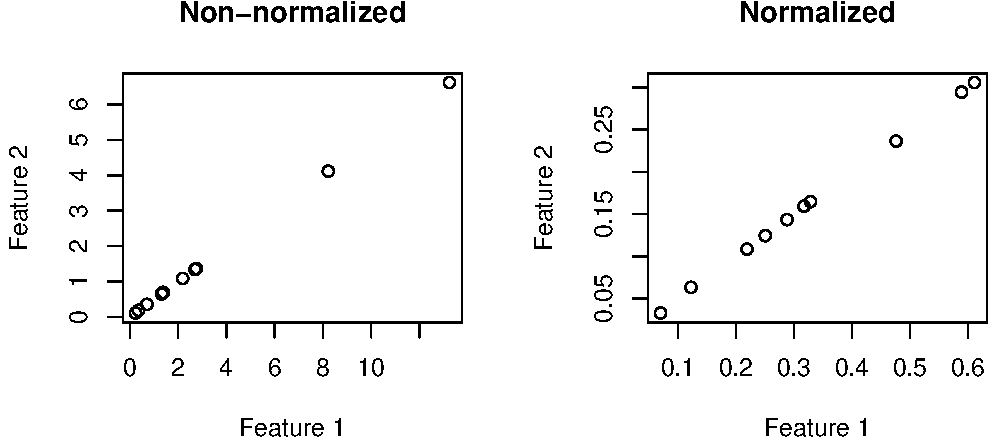
\includegraphics[width=\maxwidth]{figure/unnamed-chunk-5-1} \caption{Non-normalized and normalized associations between feature 1 and feature 2.  In this case we would expect feature 1 and feature 2 to be associated. In the output we see this by the positive sim.score value in the [1,2] element of test.output\$sim.score and the small q-value in the [1,2] element of test.output\$q.values.}\label{fig:unnamed-chunk-5}
\end{figure}
\begin{kframe}\begin{alltt}
\hlstd{test.output}
\end{alltt}
\begin{verbatim}
## $p.values
##              Feature 1    Feature 2 Feature 3  Feature 4
## Feature 1           NA 1.756616e-05 0.5654526 0.16533044
## Feature 2 1.756616e-05           NA 0.2299822 0.04276288
## Feature 3 5.654526e-01 2.299822e-01        NA 0.32957253
## Feature 4 1.653304e-01 4.276288e-02 0.3295725         NA
## 
## $z.stat
##            Feature 1 Feature 2  Feature 3  Feature 4
## Feature 1         NA  4.293774 -0.5747614 -1.3873652
## Feature 2  4.2937736        NA -1.2004047 -2.0260186
## Feature 3 -0.5747614 -1.200405         NA  0.9749753
## Feature 4 -1.3873652 -2.026019  0.9749753         NA
## 
## $sim.score
##            Feature 1  Feature 2  Feature 3  Feature 4
## Feature 1         NA  0.9999119 -0.3876728 -0.7912952
## Feature 2  0.9999119         NA -0.3859728 -0.7923909
## Feature 3 -0.3876728 -0.3859728         NA -0.2568388
## Feature 4 -0.7912952 -0.7923909 -0.2568388         NA
## 
## $q.values
##              Feature 1    Feature 2 Feature 3 Feature 4
## Feature 1           NA 0.0002496828 1.3395433 0.7833274
## Feature 2 0.0002496828           NA 0.8172331 0.3039126
## Feature 3 1.3395432651 0.8172331240        NA 0.9368990
## Feature 4 0.7833273932 0.3039125974 0.9368990        NA
\end{verbatim}
\end{kframe}
\end{knitrout}

\subsection{Example 2}

An example of how to use \Rfunction{ccrepe} with two datasets.

\begin{knitrout}
\definecolor{shadecolor}{rgb}{0.941, 0.941, 0.941}\color{fgcolor}\begin{kframe}
\begin{alltt}
\hlstd{data} \hlkwb{<-} \hlkwd{matrix}\hlstd{(}\hlkwd{rlnorm}\hlstd{(}\hlnum{40}\hlstd{,}\hlkwc{meanlog}\hlstd{=}\hlnum{0}\hlstd{,}\hlkwc{sdlog}\hlstd{=}\hlnum{1}\hlstd{),}\hlkwc{nrow}\hlstd{=}\hlnum{10}\hlstd{,}\hlkwc{ncol}\hlstd{=}\hlnum{4}\hlstd{)}
\hlstd{data[,}\hlnum{1}\hlstd{]} \hlkwb{=} \hlnum{2}\hlopt{*}\hlstd{data[,}\hlnum{2}\hlstd{]} \hlopt{+} \hlkwd{rnorm}\hlstd{(}\hlnum{10}\hlstd{,}\hlnum{0}\hlstd{,}\hlnum{0.01}\hlstd{)}
\hlstd{data.rowsum} \hlkwb{<-} \hlkwd{apply}\hlstd{(data,}\hlnum{1}\hlstd{,sum)}
\hlstd{data.norm} \hlkwb{<-} \hlstd{data}\hlopt{/}\hlstd{data.rowsum}
\hlkwd{apply}\hlstd{(data.norm,}\hlnum{1}\hlstd{,sum)}  \hlcom{# The rows sum to 1, so the data are normalized}
\end{alltt}
\begin{verbatim}
##  [1] 1 1 1 1 1 1 1 1 1 1
\end{verbatim}
\begin{alltt}
\hlstd{test.input} \hlkwb{<-} \hlstd{data.norm}


\hlstd{data2} \hlkwb{<-} \hlkwd{matrix}\hlstd{(}\hlkwd{rlnorm}\hlstd{(}\hlnum{105}\hlstd{,}\hlkwc{meanlog}\hlstd{=}\hlnum{0}\hlstd{,}\hlkwc{sdlog}\hlstd{=}\hlnum{1}\hlstd{),}\hlkwc{nrow}\hlstd{=}\hlnum{15}\hlstd{,}\hlkwc{ncol}\hlstd{=}\hlnum{7}\hlstd{)}
\hlstd{aligned.rows} \hlkwb{<-} \hlkwd{c}\hlstd{(}\hlkwd{seq}\hlstd{(}\hlnum{1}\hlstd{,}\hlnum{4}\hlstd{),}\hlkwd{seq}\hlstd{(}\hlnum{6}\hlstd{,}\hlnum{9}\hlstd{),}\hlnum{11}\hlstd{,}\hlnum{12}\hlstd{)}  \hlcom{# The datasets dont need }
                                            \hlcom{# to have subjects line up exactly}
\hlstd{data2[aligned.rows,}\hlnum{1}\hlstd{]} \hlkwb{<-}  \hlnum{2}\hlopt{*}\hlstd{data[,}\hlnum{3}\hlstd{]} \hlopt{+} \hlkwd{rnorm}\hlstd{(}\hlnum{10}\hlstd{,}\hlnum{0}\hlstd{,}\hlnum{0.01}\hlstd{)}
\hlstd{data2.rowsum} \hlkwb{<-} \hlkwd{apply}\hlstd{(data2,}\hlnum{1}\hlstd{,sum)}
\hlstd{data2.norm} \hlkwb{<-} \hlstd{data2}\hlopt{/}\hlstd{data2.rowsum}
\hlkwd{apply}\hlstd{(data2.norm,}\hlnum{1}\hlstd{,sum)}  \hlcom{# The rows sum to 1, so the data are normalized}
\end{alltt}
\begin{verbatim}
##  [1] 1 1 1 1 1 1 1 1 1 1 1 1 1 1 1
\end{verbatim}
\begin{alltt}
\hlstd{test.input.2} \hlkwb{<-} \hlstd{data2.norm}

\hlkwd{dimnames}\hlstd{(test.input)} \hlkwb{<-} \hlkwd{list}\hlstd{(}\hlkwd{paste}\hlstd{(}\hlstr{"Sample"}\hlstd{,}\hlkwd{seq}\hlstd{(}\hlnum{1}\hlstd{,}\hlnum{10}\hlstd{)),}\hlkwd{paste}\hlstd{(}\hlstr{"Feature"}\hlstd{,}\hlkwd{seq}\hlstd{(}\hlnum{1}\hlstd{,}\hlnum{4}\hlstd{)))}
\hlkwd{dimnames}\hlstd{(test.input.2)} \hlkwb{<-} \hlkwd{list}\hlstd{(}\hlkwd{paste}\hlstd{(}\hlstr{"Sample"}\hlstd{,}\hlkwd{c}\hlstd{(}\hlkwd{seq}\hlstd{(}\hlnum{1}\hlstd{,}\hlnum{4}\hlstd{),}\hlnum{11}\hlstd{,}\hlkwd{seq}\hlstd{(}\hlnum{5}\hlstd{,}\hlnum{8}\hlstd{),}\hlnum{12}\hlstd{,}\hlnum{9}\hlstd{,}\hlnum{10}\hlstd{,}\hlnum{13}\hlstd{,}\hlnum{14}\hlstd{,}\hlnum{15}\hlstd{)),}\hlkwd{paste}\hlstd{(}\hlstr{"Feature"}\hlstd{,}\hlkwd{seq}\hlstd{(}\hlnum{1}\hlstd{,}\hlnum{7}\hlstd{)))}

\hlstd{test.output.two.datasets} \hlkwb{<-} \hlkwd{ccrepe}\hlstd{(}\hlkwc{x}\hlstd{=test.input,} \hlkwc{y}\hlstd{=test.input.2,} \hlkwc{iterations}\hlstd{=}\hlnum{20}\hlstd{,} \hlkwc{min.subj}\hlstd{=}\hlnum{10}\hlstd{)}
\end{alltt}


{\ttfamily\noindent\color{warningcolor}{\#\# Warning in preprocess\_data(CA): Removing subjects Sample 11, Sample 12, Sample 13, Sample 14, Sample 15 from dataset y because they are not in dataset x.}}\end{kframe}
\end{knitrout}
Please note that we receive a warning because the subjects don't match - only paired observations.
 
\begin{knitrout}
\definecolor{shadecolor}{rgb}{0.941, 0.941, 0.941}\color{fgcolor}\begin{kframe}
\begin{alltt}
\hlkwd{par}\hlstd{(}\hlkwc{mfrow}\hlstd{=}\hlkwd{c}\hlstd{(}\hlnum{1}\hlstd{,}\hlnum{2}\hlstd{))}
\hlkwd{plot}\hlstd{(data2[aligned.rows,}\hlnum{1}\hlstd{],data[,}\hlnum{3}\hlstd{],}\hlkwc{xlab}\hlstd{=}\hlstr{"dataset 2: Feature 1"}\hlstd{,}\hlkwc{ylab}\hlstd{=}\hlstr{"dataset 1: Feature 3"}\hlstd{,}\hlkwc{main}\hlstd{=}\hlstr{"Non-normalized"}\hlstd{)}
\hlkwd{plot}\hlstd{(data2.norm[aligned.rows,}\hlnum{1}\hlstd{],data.norm[,}\hlnum{3}\hlstd{],}\hlkwc{xlab}\hlstd{=}\hlstr{"dataset 2: Feature 1"}\hlstd{,}\hlkwc{ylab}\hlstd{=}\hlstr{"dataset 1: Feature 3"}\hlstd{,}
     \hlkwc{main}\hlstd{=}\hlstr{"Normalized"}\hlstd{)}
\end{alltt}
\end{kframe}\begin{figure}[H]
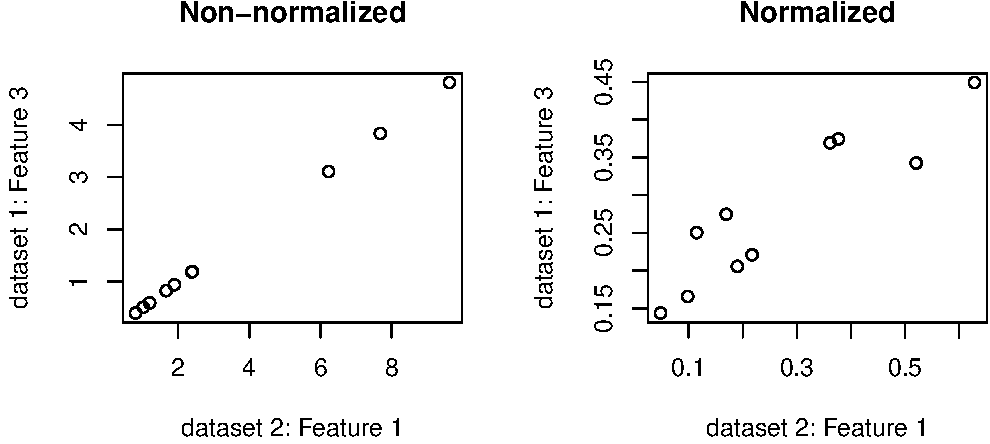
\includegraphics[width=\maxwidth]{figure/unnamed-chunk-7-1} \caption{Non-normalized and normalized associations between feature 1 and feature 2.  In this case we would expect feature 1 and feature 2 to be associated. In the output we see this by the positive sim.score value in the [1,2] element of test.output\$sim.score and the small q-value in the [1,2] element of test.output\$q.values.}\label{fig:unnamed-chunk-7}
\end{figure}
\begin{kframe}\begin{alltt}
\hlstd{test.output.two.datasets}
\end{alltt}
\begin{verbatim}
## $p.values
##             Feature 1   Feature 2 Feature 3 Feature 4  Feature 5 Feature 6
## Feature 1 0.345872402 0.419383416 0.9432693 0.5006452 0.35064584 0.2216574
## Feature 2 0.265286949 0.371659168 0.8074678 0.4084374 0.37293944 0.1756130
## Feature 3 0.002050669 0.005449224 0.3733573 0.7184186 0.22331262 0.6460115
## Feature 4 0.740295138 0.511050407 0.7169565 0.3534291 0.07328915 0.3795741
##            Feature 7
## Feature 1 0.96084739
## Feature 2 0.89331951
## Feature 3 0.07237619
## Feature 4 0.53927351
## 
## $z.stat
##            Feature 1  Feature 2   Feature 3  Feature 4  Feature 5  Feature 6
## Feature 1 -0.9426257  0.8074914  0.07116139  0.6734749  0.9333373 -1.2221327
## Feature 2 -1.1139819  0.8933698 -0.24369396  0.8266465  0.8909809 -1.3543869
## Feature 3  3.0827942 -2.7792043 -0.89020227  0.3605731  1.2177667  0.4593101
## Feature 4 -0.3314625  0.6572030  0.36252939 -0.9279585 -1.7910259  0.8786813
##             Feature 7
## Feature 1  0.04909023
## Feature 2  0.13410505
## Feature 3 -1.79674451
## Feature 4  0.61391195
## 
## $sim.score
##             Feature 1   Feature 2   Feature 3    Feature 4  Feature 5
## Feature 1 -0.39577927  0.26949793 -0.07841653  0.196328360  0.3438109
## Feature 2 -0.39946820  0.26984242 -0.07808791  0.198252113  0.3426280
## Feature 3  0.91139207 -0.63408844 -0.25676915 -0.006946768  0.2964227
## Feature 4 -0.06748179  0.05391557  0.21966731 -0.204136706 -0.5205751
##            Feature 6   Feature 7
## Feature 1 -0.4029356  0.17725578
## Feature 2 -0.4043042  0.18336066
## Feature 3  0.1025558 -0.46187735
## Feature 4  0.3709278  0.05731246
## 
## $q.values
##           Feature 1 Feature 2 Feature 3 Feature 4 Feature 5 Feature 6
## Feature 1  4.206722 2.7004287  3.824215  3.044584  3.838301  4.043910
## Feature 2  3.629914 3.3902677  3.535539  2.794319  3.140258  3.844652
## Feature 3  0.224474 0.2982463  2.919221  3.419165  3.492092  3.367374
## Feature 4  3.376479 2.9442896  3.567307  3.517062  2.005626  2.769974
##           Feature 7
## Feature 1  3.756356
## Feature 2  3.761004
## Feature 3  2.640857
## Feature 4  2.951545
\end{verbatim}
\end{kframe}
\end{knitrout}

\subsection{Example 3}

An example of how to use \Rfunction{ccrepe} with \Rfunction{nc.score} as the similarity score.

\begin{knitrout}
\definecolor{shadecolor}{rgb}{0.941, 0.941, 0.941}\color{fgcolor}\begin{kframe}
\begin{alltt}
\hlstd{data} \hlkwb{<-} \hlkwd{matrix}\hlstd{(}\hlkwd{rlnorm}\hlstd{(}\hlnum{40}\hlstd{,}\hlkwc{meanlog}\hlstd{=}\hlnum{0}\hlstd{,}\hlkwc{sdlog}\hlstd{=}\hlnum{1}\hlstd{),}\hlkwc{nrow}\hlstd{=}\hlnum{10}\hlstd{,}\hlkwc{ncol}\hlstd{=}\hlnum{4}\hlstd{)}
\hlstd{data[,}\hlnum{1}\hlstd{]} \hlkwb{=} \hlnum{2}\hlopt{*}\hlstd{data[,}\hlnum{2}\hlstd{]} \hlopt{+} \hlkwd{rnorm}\hlstd{(}\hlnum{10}\hlstd{,}\hlnum{0}\hlstd{,}\hlnum{0.01}\hlstd{)}
\hlstd{data.rowsum} \hlkwb{<-} \hlkwd{apply}\hlstd{(data,}\hlnum{1}\hlstd{,sum)}
\hlstd{data.norm} \hlkwb{<-} \hlstd{data}\hlopt{/}\hlstd{data.rowsum}
\hlkwd{apply}\hlstd{(data.norm,}\hlnum{1}\hlstd{,sum)}  \hlcom{# The rows sum to 1, so the data are normalized}
\end{alltt}
\begin{verbatim}
##  [1] 1 1 1 1 1 1 1 1 1 1
\end{verbatim}
\begin{alltt}
\hlstd{test.input} \hlkwb{<-} \hlstd{data.norm}

\hlkwd{dimnames}\hlstd{(test.input)} \hlkwb{<-} \hlkwd{list}\hlstd{(}\hlkwd{paste}\hlstd{(}\hlstr{"Sample"}\hlstd{,}\hlkwd{seq}\hlstd{(}\hlnum{1}\hlstd{,}\hlnum{10}\hlstd{)),}\hlkwd{paste}\hlstd{(}\hlstr{"Feature"}\hlstd{,}\hlkwd{seq}\hlstd{(}\hlnum{1}\hlstd{,}\hlnum{4}\hlstd{)))}

\hlstd{test.output.nc.score}     \hlkwb{<-} \hlkwd{ccrepe}\hlstd{(}\hlkwc{x}\hlstd{=test.input,} \hlkwc{sim.score}\hlstd{=nc.score,} \hlkwc{iterations}\hlstd{=}\hlnum{20}\hlstd{,} \hlkwc{min.subj}\hlstd{=}\hlnum{10}\hlstd{)}
\end{alltt}
\end{kframe}
\end{knitrout}
\begin{knitrout}
\definecolor{shadecolor}{rgb}{0.941, 0.941, 0.941}\color{fgcolor}\begin{kframe}
\begin{alltt}
\hlkwd{par}\hlstd{(}\hlkwc{mfrow}\hlstd{=}\hlkwd{c}\hlstd{(}\hlnum{1}\hlstd{,}\hlnum{2}\hlstd{))}
\hlkwd{plot}\hlstd{(data[,}\hlnum{1}\hlstd{],data[,}\hlnum{2}\hlstd{],}\hlkwc{xlab}\hlstd{=}\hlstr{"Feature 1"}\hlstd{,}\hlkwc{ylab}\hlstd{=}\hlstr{"Feature 2"}\hlstd{,}\hlkwc{main}\hlstd{=}\hlstr{"Non-normalized"}\hlstd{)}
\hlkwd{plot}\hlstd{(data.norm[,}\hlnum{1}\hlstd{],data.norm[,}\hlnum{2}\hlstd{],}\hlkwc{xlab}\hlstd{=}\hlstr{"Feature 1"}\hlstd{,}\hlkwc{ylab}\hlstd{=}\hlstr{"Feature 2"}\hlstd{,}
     \hlkwc{main}\hlstd{=}\hlstr{"Normalized"}\hlstd{)}
\end{alltt}
\end{kframe}\begin{figure}[H]
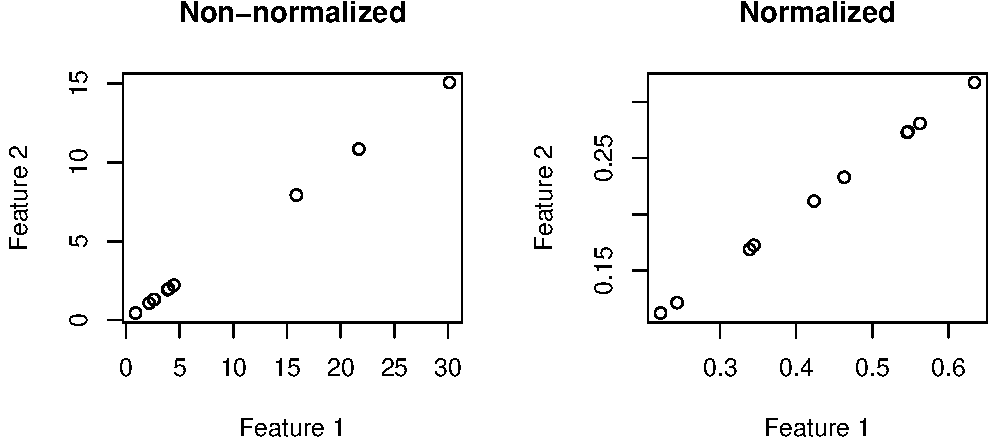
\includegraphics[width=\maxwidth]{figure/unnamed-chunk-9-1} \caption{Non-normalized and normalized associations between feature 1 and feature 2.  In this case we would expect feature 1 and feature 2 to be associated. In the output we see this by the positive sim.score value in the [1,2] element of test.output\$sim.score and the small q-value in the [1,2] element of test.output\$q.values. In this case, however, the sim.score represents the NC-Score between two features rather than the Spearman correlation.}\label{fig:unnamed-chunk-9}
\end{figure}
\begin{kframe}\begin{alltt}
\hlstd{test.output.nc.score}
\end{alltt}
\begin{verbatim}
## $p.values
##              Feature 1    Feature 2 Feature 3 Feature 4
## Feature 1           NA 2.842233e-06 0.4112287 0.6724454
## Feature 2 2.842233e-06           NA 0.2225533 0.2176691
## Feature 3 4.112287e-01 2.225533e-01        NA 0.4681866
## Feature 4 6.724454e-01 2.176691e-01 0.4681866        NA
## 
## $z.stat
##            Feature 1 Feature 2  Feature 3  Feature 4
## Feature 1         NA  4.681903 -0.8217333 -0.4227942
## Feature 2  4.6819035        NA -1.2197667 -1.2327499
## Feature 3 -0.8217333 -1.219767         NA  0.7254327
## Feature 4 -0.4227942 -1.232750  0.7254327         NA
## 
## $sim.score
##           Feature 1 Feature 2 Feature 3 Feature 4
## Feature 1        NA   1.00000   -0.4375  -0.59375
## Feature 2   1.00000        NA   -0.4375  -0.59375
## Feature 3  -0.43750  -0.43750        NA   0.00000
## Feature 4  -0.59375  -0.59375    0.0000        NA
## 
## $q.values
##              Feature 1    Feature 2 Feature 3 Feature 4
## Feature 1           NA 4.039908e-05  1.461286  1.593006
## Feature 2 4.039908e-05           NA  1.054447  1.546958
## Feature 3 1.461286e+00 1.054447e+00        NA  1.330947
## Feature 4 1.593006e+00 1.546958e+00  1.330947        NA
\end{verbatim}
\end{kframe}
\end{knitrout}

\subsection{Example 4}

An example of how to use \Rfunction{ccrepe} with a user-defined \Rfunction{sim.score} function.

\begin{knitrout}
\definecolor{shadecolor}{rgb}{0.941, 0.941, 0.941}\color{fgcolor}\begin{kframe}
\begin{alltt}
\hlstd{data} \hlkwb{<-} \hlkwd{matrix}\hlstd{(}\hlkwd{rlnorm}\hlstd{(}\hlnum{40}\hlstd{,}\hlkwc{meanlog}\hlstd{=}\hlnum{0}\hlstd{,}\hlkwc{sdlog}\hlstd{=}\hlnum{1}\hlstd{),}\hlkwc{nrow}\hlstd{=}\hlnum{10}\hlstd{,}\hlkwc{ncol}\hlstd{=}\hlnum{4}\hlstd{)}
\hlstd{data[,}\hlnum{1}\hlstd{]} \hlkwb{=} \hlnum{2}\hlopt{*}\hlstd{data[,}\hlnum{2}\hlstd{]} \hlopt{+} \hlkwd{rnorm}\hlstd{(}\hlnum{10}\hlstd{,}\hlnum{0}\hlstd{,}\hlnum{0.01}\hlstd{)}
\hlstd{data.rowsum} \hlkwb{<-} \hlkwd{apply}\hlstd{(data,}\hlnum{1}\hlstd{,sum)}
\hlstd{data.norm} \hlkwb{<-} \hlstd{data}\hlopt{/}\hlstd{data.rowsum}
\hlkwd{apply}\hlstd{(data.norm,}\hlnum{1}\hlstd{,sum)}  \hlcom{# The rows sum to 1, so the data are normalized}
\end{alltt}
\begin{verbatim}
##  [1] 1 1 1 1 1 1 1 1 1 1
\end{verbatim}
\begin{alltt}
\hlstd{test.input} \hlkwb{<-} \hlstd{data.norm}

\hlkwd{dimnames}\hlstd{(test.input)} \hlkwb{<-} \hlkwd{list}\hlstd{(}\hlkwd{paste}\hlstd{(}\hlstr{"Sample"}\hlstd{,}\hlkwd{seq}\hlstd{(}\hlnum{1}\hlstd{,}\hlnum{10}\hlstd{)),}\hlkwd{paste}\hlstd{(}\hlstr{"Feature"}\hlstd{,}\hlkwd{seq}\hlstd{(}\hlnum{1}\hlstd{,}\hlnum{4}\hlstd{)))}

\hlstd{my.test.sim.score} \hlkwb{<-} \hlkwa{function}\hlstd{(}\hlkwc{x}\hlstd{,}\hlkwc{y}\hlstd{=}\hlnum{NA}\hlstd{,}\hlkwc{constant}\hlstd{=}\hlnum{0.5}\hlstd{)\{}
       \hlkwa{if}\hlstd{(}\hlkwd{is.vector}\hlstd{(x)} \hlopt{&&} \hlkwd{is.vector}\hlstd{(y))} \hlkwd{return}\hlstd{(constant)}
          \hlkwa{if}\hlstd{(}\hlkwd{is.matrix}\hlstd{(x)} \hlopt{&&} \hlkwd{is.na}\hlstd{(y))} \hlkwd{return}\hlstd{(}\hlkwd{matrix}\hlstd{(}\hlkwd{rep}\hlstd{(constant,}\hlkwd{ncol}\hlstd{(x)}\hlopt{^}\hlnum{2}\hlstd{),}\hlkwc{ncol}\hlstd{=}\hlkwd{ncol}\hlstd{(x)))}
          \hlkwa{if}\hlstd{(}\hlkwd{is.data.frame}\hlstd{(x)} \hlopt{&&} \hlkwd{is.na}\hlstd{(y))} \hlkwd{return}\hlstd{(}\hlkwd{matrix}\hlstd{(}\hlkwd{rep}\hlstd{(constant,}\hlkwd{ncol}\hlstd{(x)}\hlopt{^}\hlnum{2}\hlstd{),}\hlkwc{ncol}\hlstd{=}\hlkwd{ncol}\hlstd{(x)))}
          \hlkwa{else} \hlkwd{stop}\hlstd{(}\hlstr{'ERROR'}\hlstd{)}
   \hlstd{\}}

\hlstd{test.output.sim.score}    \hlkwb{<-} \hlkwd{ccrepe}\hlstd{(}\hlkwc{x}\hlstd{=test.input,} \hlkwc{sim.score}\hlstd{=my.test.sim.score,} \hlkwc{iterations}\hlstd{=}\hlnum{20}\hlstd{,} \hlkwc{min.subj}\hlstd{=}\hlnum{10}\hlstd{,} \hlkwc{sim.score.args} \hlstd{=} \hlkwd{list}\hlstd{(}\hlkwc{constant} \hlstd{=} \hlnum{0.6}\hlstd{))}
\end{alltt}
\end{kframe}
\end{knitrout}
\begin{knitrout}
\definecolor{shadecolor}{rgb}{0.941, 0.941, 0.941}\color{fgcolor}\begin{kframe}
\begin{alltt}
\hlkwd{par}\hlstd{(}\hlkwc{mfrow}\hlstd{=}\hlkwd{c}\hlstd{(}\hlnum{1}\hlstd{,}\hlnum{2}\hlstd{))}
\hlkwd{plot}\hlstd{(data[,}\hlnum{1}\hlstd{],data[,}\hlnum{2}\hlstd{],}\hlkwc{xlab}\hlstd{=}\hlstr{"Feature 1"}\hlstd{,}\hlkwc{ylab}\hlstd{=}\hlstr{"Feature 2"}\hlstd{,}\hlkwc{main}\hlstd{=}\hlstr{"Non-normalized"}\hlstd{)}
\hlkwd{plot}\hlstd{(data.norm[,}\hlnum{1}\hlstd{],data.norm[,}\hlnum{2}\hlstd{],}\hlkwc{xlab}\hlstd{=}\hlstr{"Feature 1"}\hlstd{,}\hlkwc{ylab}\hlstd{=}\hlstr{"Feature 2"}\hlstd{,}
     \hlkwc{main}\hlstd{=}\hlstr{"Normalized"}\hlstd{)}
\end{alltt}
\end{kframe}\begin{figure}[H]
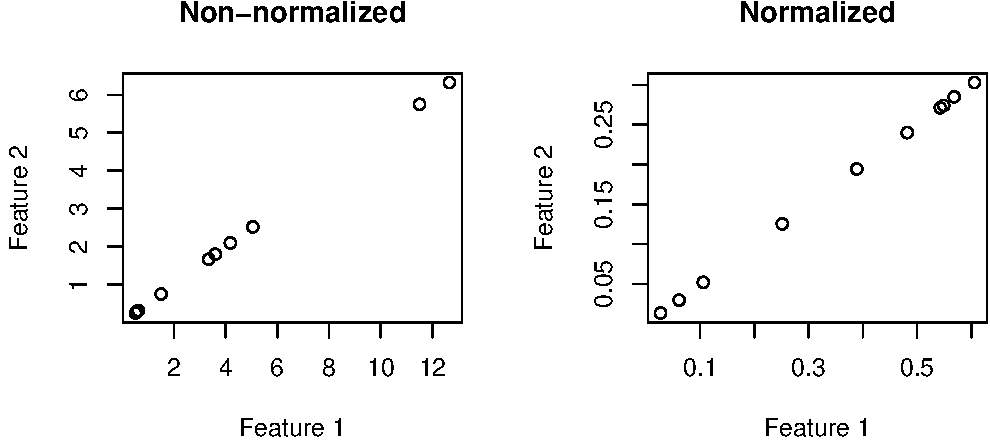
\includegraphics[width=\maxwidth]{figure/unnamed-chunk-11-1} \caption{Non-normalized and normalized associations between feature 1 and feature 2.  In this case we would expect feature 1 and feature 2 to be associated. Note that the values of sim.score are all 0.6 and none of the p-values are very small because of the arbitrary definition of the similarity score.}\label{fig:unnamed-chunk-11}
\end{figure}
\begin{kframe}\begin{alltt}
\hlstd{test.output.sim.score}
\end{alltt}
\begin{verbatim}
## $p.values
##           Feature 1 Feature 2 Feature 3 Feature 4
## Feature 1        NA       NaN       NaN       NaN
## Feature 2       NaN        NA       NaN       NaN
## Feature 3       NaN       NaN        NA       NaN
## Feature 4       NaN       NaN       NaN        NA
## 
## $z.stat
##           Feature 1 Feature 2 Feature 3 Feature 4
## Feature 1        NA       NaN       NaN       NaN
## Feature 2       NaN        NA       NaN       NaN
## Feature 3       NaN       NaN        NA       NaN
## Feature 4       NaN       NaN       NaN        NA
## 
## $sim.score
##           Feature 1 Feature 2 Feature 3 Feature 4
## Feature 1        NA       0.6       0.6       0.6
## Feature 2       0.6        NA       0.6       0.6
## Feature 3       0.6       0.6        NA       0.6
## Feature 4       0.6       0.6       0.6        NA
## 
## $q.values
##           Feature 1 Feature 2 Feature 3 Feature 4
## Feature 1        NA       NaN       NaN       NaN
## Feature 2       NaN        NA       NaN       NaN
## Feature 3       NaN       NaN        NA       NaN
## Feature 4       NaN       NaN       NaN        NA
\end{verbatim}
\end{kframe}
\end{knitrout}

\subsection{Example 5}

An example of how to use \Rfunction{ccrepe} when specifying column subsets.

\begin{knitrout}
\definecolor{shadecolor}{rgb}{0.941, 0.941, 0.941}\color{fgcolor}\begin{kframe}
\begin{alltt}
\hlstd{data} \hlkwb{<-} \hlkwd{matrix}\hlstd{(}\hlkwd{rlnorm}\hlstd{(}\hlnum{40}\hlstd{,}\hlkwc{meanlog}\hlstd{=}\hlnum{0}\hlstd{,}\hlkwc{sdlog}\hlstd{=}\hlnum{1}\hlstd{),}\hlkwc{nrow}\hlstd{=}\hlnum{10}\hlstd{,}\hlkwc{ncol}\hlstd{=}\hlnum{4}\hlstd{)}
\hlstd{data.rowsum} \hlkwb{<-} \hlkwd{apply}\hlstd{(data,}\hlnum{1}\hlstd{,sum)}
\hlstd{data.norm} \hlkwb{<-} \hlstd{data}\hlopt{/}\hlstd{data.rowsum}
\hlkwd{apply}\hlstd{(data.norm,}\hlnum{1}\hlstd{,sum)}  \hlcom{# The rows sum to 1, so the data are normalized}
\end{alltt}
\begin{verbatim}
##  [1] 1 1 1 1 1 1 1 1 1 1
\end{verbatim}
\begin{alltt}
\hlstd{test.input} \hlkwb{<-} \hlstd{data.norm}

\hlkwd{dimnames}\hlstd{(test.input)} \hlkwb{<-} \hlkwd{list}\hlstd{(}\hlkwd{paste}\hlstd{(}\hlstr{"Sample"}\hlstd{,}\hlkwd{seq}\hlstd{(}\hlnum{1}\hlstd{,}\hlnum{10}\hlstd{)),}\hlkwd{paste}\hlstd{(}\hlstr{"Feature"}\hlstd{,}\hlkwd{seq}\hlstd{(}\hlnum{1}\hlstd{,}\hlnum{4}\hlstd{)))}

\hlstd{test.output.1.3}     \hlkwb{<-} \hlkwd{ccrepe}\hlstd{(}\hlkwc{x}\hlstd{=test.input,} \hlkwc{iterations}\hlstd{=}\hlnum{20}\hlstd{,} \hlkwc{min.subj}\hlstd{=}\hlnum{10}\hlstd{,} \hlkwc{subset.cols.x}\hlstd{=}\hlkwd{c}\hlstd{(}\hlnum{1}\hlstd{,}\hlnum{3}\hlstd{))}
\hlstd{test.output.1}       \hlkwb{<-} \hlkwd{ccrepe}\hlstd{(}\hlkwc{x}\hlstd{=test.input,} \hlkwc{iterations}\hlstd{=}\hlnum{20}\hlstd{,} \hlkwc{min.subj}\hlstd{=}\hlnum{10}\hlstd{,} \hlkwc{subset.cols.x}\hlstd{=}\hlkwd{c}\hlstd{(}\hlnum{1}\hlstd{),} \hlkwc{compare.within.x}\hlstd{=}\hlnum{FALSE}\hlstd{)}
\hlstd{test.output.12.3}    \hlkwb{<-} \hlkwd{ccrepe}\hlstd{(}\hlkwc{x}\hlstd{=test.input,} \hlkwc{iterations}\hlstd{=}\hlnum{20}\hlstd{,} \hlkwc{min.subj}\hlstd{=}\hlnum{10}\hlstd{,} \hlkwc{subset.cols.x}\hlstd{=}\hlkwd{c}\hlstd{(}\hlnum{1}\hlstd{,}\hlnum{2}\hlstd{),}\hlkwc{subset.cols.y}\hlstd{=}\hlkwd{c}\hlstd{(}\hlnum{3}\hlstd{),} \hlkwc{compare.within.x}\hlstd{=}\hlnum{FALSE}\hlstd{)}
\hlstd{test.output.1.3}\hlopt{$}\hlstd{sim.score}
\end{alltt}
\begin{verbatim}
##            Feature 1  Feature 3
## Feature 1         NA -0.2057674
## Feature 3 -0.2057674         NA
\end{verbatim}
\begin{alltt}
\hlstd{test.output.1}\hlopt{$}\hlstd{sim.score}
\end{alltt}
\begin{verbatim}
##            Feature 1  Feature 2  Feature 3  Feature 4
## Feature 1         NA -0.4314052 -0.2057674 -0.5379471
## Feature 2 -0.4314052         NA         NA         NA
## Feature 3 -0.2057674         NA         NA         NA
## Feature 4 -0.5379471         NA         NA         NA
\end{verbatim}
\begin{alltt}
\hlstd{test.output.12.3}\hlopt{$}\hlstd{sim.score}
\end{alltt}
\begin{verbatim}
##            Feature 1  Feature 2  Feature 3 Feature 4
## Feature 1         NA         NA -0.2057674        NA
## Feature 2         NA         NA -0.1505928        NA
## Feature 3 -0.2057674 -0.1505928         NA        NA
## Feature 4         NA         NA         NA        NA
\end{verbatim}
\end{kframe}
\end{knitrout}

%---------------------------------------------------------
\section{nc.score} 
%---------------------------------------------------------

The \Rfunction{nc.score} similarity measure is an N-dimensional extension of the checkerboard score particularly suited to similarity score calculations between compositions derived from ecological relative abundance measurements.  In such cases, features typically represent species abundances, and the NC-score discretizes these continuous values into one of N bins before computing a normalized similarity of co-occurrence or co-exclusion.  This can be used as a standalone function or with \Rfunction{ccrepe} as above to obtain compositionality-corrected p-values.

\subsection{General Functionality}

The NC-score is an extension to Diamond's checkerboard score (see \citet{cody1975ecology}) to ordinal data, and simplifies to a calculation of Kendall's $\tau$ on binned data instead of ranked data.  Let two features in a dataset with $n$ subjects be denoted by
\[
\left[ \begin{array}{cccc}
    x_1 & x_2 & \dots & x_n\\
    y_1 & y_2 & \dots & y_n\\
    \end{array} \right].
\]
The binning function maps from the original data to $b$ numbered bins in $\{1,...,b\}$.  Let the binning function be denoted by $B(\cdot)$. The co-variation and co-exclusion patterns are the same as concordant and discordant pairs in Kendall's $\tau$.  Considering a $2 \times 2$ submatrix of the form
\[
\left[ \begin{array}{cc}
    B(x_i) & B(x_j)\\
    B(y_i) & B(y_j)\\
    \end{array} \right],
\]
a co-variation pattern is counted when $(B(x_i) - B(x_j))(B(y_i) - B(y_j)) > 0$ and a co-exclusion pattern, conversely, when $(B(x_i) - B(x_j))(B(y_i) - B(y_j)) < 0$.  The NC-score statistic for features $x$ and $y$ is then defined as 
\[
(\text{number of co-variation patterns}) - (\text{number of co-exclusion patterns}),
\]
normalized by the Kendall's $\tau$ normalization factor accounting for ties described in \citet{kendall1970}.

\subsection{Arguments}

\begin{description}
\setlength{\itemsep}{1em}

\item[\Rcode{x}]
First numerical \Rclass{vector}, or single \Rclass{dataframe} or \Rclass{matrix}, containing relative abundances.  If the latter, columns are features, rows are samples.  Rows should therefore sum to a constant.

\item[\Rcode{y}]
If provided, second numerical \Rclass{vector} containing relative abundances.  If given, \Rcode{x} must be a \Rclass{vector} as well.

\item[\Rcode{nbins}]
A non-negative integer of the number of bins to generate (cutoffs will be generated by the discretize function from the infotheo package).
 
\item[\Rcode{bin.cutoffs}]
A list of values demarcating the bin cutoffs.  The binning is   performed using the findInterval function.

\item[\Rcode{use}]
An optional character string givinga method for computing covariances    in the presence of missing values.  This must be (an abbreviaion of) on of the strings "everything", "all.obs", "complete.obs","na.or.complete", or "pairwise.complete.obs".

\end{description}

\subsection{Output}

\Rfunction{nc.score} returns either a single number (if called with two vectors) or a \Rclass{matrix} of all pairwise scores (if called with a \Rclass{matrix}) of normalized scores.
This behaviour is precisely analogous to the cor function in R


\subsection{Usage}

\begin{knitrout}
\definecolor{shadecolor}{rgb}{0.941, 0.941, 0.941}\color{fgcolor}\begin{kframe}
\begin{alltt}
\hlkwd{nc.score}\hlstd{(}
 \hlstd{x,}
 \hlkwc{y} \hlstd{=} \hlkwa{NULL}\hlstd{,}
 \hlkwc{use} \hlstd{=} \hlstr{"everything"}\hlstd{,}
 \hlkwc{nbins} \hlstd{=} \hlkwa{NULL}\hlstd{,}
 \hlkwc{bin.cutoffs}\hlstd{=}\hlkwa{NULL}\hlstd{)}
\end{alltt}
\end{kframe}
\end{knitrout}

\subsection{Example 1}

An example of using \Rfunction{nc.score} to get a single similarity score or a matrix.

\begin{knitrout}
\definecolor{shadecolor}{rgb}{0.941, 0.941, 0.941}\color{fgcolor}\begin{kframe}
\begin{alltt}
\hlstd{data} \hlkwb{<-} \hlkwd{matrix}\hlstd{(}\hlkwd{rlnorm}\hlstd{(}\hlnum{40}\hlstd{,}\hlkwc{meanlog}\hlstd{=}\hlnum{0}\hlstd{,}\hlkwc{sdlog}\hlstd{=}\hlnum{1}\hlstd{),}\hlkwc{nrow}\hlstd{=}\hlnum{10}\hlstd{,}\hlkwc{ncol}\hlstd{=}\hlnum{4}\hlstd{)}
\hlstd{data.rowsum} \hlkwb{<-} \hlkwd{apply}\hlstd{(data,}\hlnum{1}\hlstd{,sum)}
\hlstd{data[,}\hlnum{1}\hlstd{]} \hlkwb{=} \hlnum{2}\hlopt{*}\hlstd{data[,}\hlnum{2}\hlstd{]} \hlopt{+} \hlkwd{rnorm}\hlstd{(}\hlnum{10}\hlstd{,}\hlnum{0}\hlstd{,}\hlnum{0.01}\hlstd{)}
\hlstd{data.norm} \hlkwb{<-} \hlstd{data}\hlopt{/}\hlstd{data.rowsum}
\hlkwd{apply}\hlstd{(data.norm,}\hlnum{1}\hlstd{,sum)}  \hlcom{# The rows sum to 1, so the data are normalized}
\end{alltt}
\begin{verbatim}
##  [1] 0.3920407 0.9723630 1.3591161 0.6423790 0.8270197 1.0181079 0.6733859
##  [8] 1.3173995 0.9984763 0.5751192
\end{verbatim}
\begin{alltt}
\hlstd{test.input} \hlkwb{<-} \hlstd{data.norm}

\hlkwd{dimnames}\hlstd{(test.input)} \hlkwb{<-} \hlkwd{list}\hlstd{(}\hlkwd{paste}\hlstd{(}\hlstr{"Sample"}\hlstd{,}\hlkwd{seq}\hlstd{(}\hlnum{1}\hlstd{,}\hlnum{10}\hlstd{)),}\hlkwd{paste}\hlstd{(}\hlstr{"Feature"}\hlstd{,}\hlkwd{seq}\hlstd{(}\hlnum{1}\hlstd{,}\hlnum{4}\hlstd{)))}

\hlstd{test.output.matrix} \hlkwb{<-} \hlkwd{nc.score}\hlstd{(}\hlkwc{x}\hlstd{=test.input)}
\hlstd{test.output.num}    \hlkwb{<-} \hlkwd{nc.score}\hlstd{(}\hlkwc{x}\hlstd{=test.input[,}\hlnum{1}\hlstd{],}\hlkwc{y}\hlstd{=test.input[,}\hlnum{2}\hlstd{])}
\end{alltt}
\end{kframe}
\end{knitrout}
\begin{knitrout}
\definecolor{shadecolor}{rgb}{0.941, 0.941, 0.941}\color{fgcolor}\begin{kframe}
\begin{alltt}
\hlkwd{par}\hlstd{(}\hlkwc{mfrow}\hlstd{=}\hlkwd{c}\hlstd{(}\hlnum{1}\hlstd{,} \hlnum{2}\hlstd{))}
\hlkwd{plot}\hlstd{(data[,}\hlnum{1}\hlstd{],data[,}\hlnum{2}\hlstd{],}\hlkwc{xlab}\hlstd{=}\hlstr{"Feature 1"}\hlstd{,}\hlkwc{ylab}\hlstd{=}\hlstr{"Feature 2"}\hlstd{,}\hlkwc{main}\hlstd{=}\hlstr{"Non-normalized"}\hlstd{)}
\hlkwd{plot}\hlstd{(data.norm[,}\hlnum{1}\hlstd{],data.norm[,}\hlnum{2}\hlstd{],}\hlkwc{xlab}\hlstd{=}\hlstr{"Feature 1"}\hlstd{,}\hlkwc{ylab}\hlstd{=}\hlstr{"Feature 2"}\hlstd{,}
     \hlkwc{main}\hlstd{=}\hlstr{"Normalized"}\hlstd{)}
\end{alltt}
\end{kframe}\begin{figure}[H]
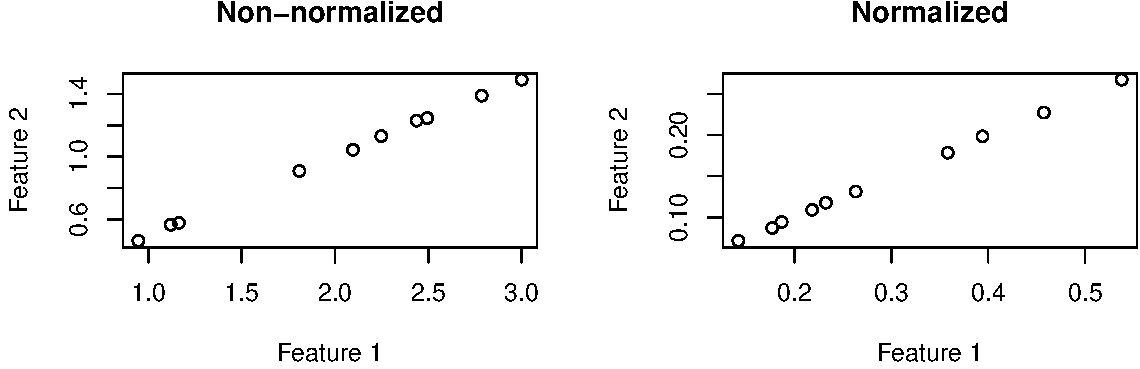
\includegraphics[width=\maxwidth]{figure/unnamed-chunk-14-1} \caption{Non-normalized and normalized associations between feature 1 and feature 2 of the second example.  Again, we expect to observe a positive association between feature 1 and feature 2.  In terms of generalized checkerboard scores, we would expect to see more co-variation patterns than co-exclusion patterns.  This is shown by the positive and relatively high value of the [1,2] element of test.output.matrix (which is identical to test.output.num)}\label{fig:unnamed-chunk-14}
\end{figure}
\begin{kframe}\begin{alltt}
\hlstd{test.output.matrix}
\end{alltt}
\begin{verbatim}
##           Feature 1 Feature 2 Feature 3 Feature 4
## Feature 1   1.00000   1.00000   0.21875   0.43750
## Feature 2   1.00000   1.00000   0.21875   0.43750
## Feature 3   0.21875   0.21875   1.00000   0.34375
## Feature 4   0.43750   0.43750   0.34375   1.00000
\end{verbatim}
\begin{alltt}
\hlstd{test.output.num}
\end{alltt}
\begin{verbatim}
## [1] 1
\end{verbatim}
\end{kframe}
\end{knitrout}

\subsection{Example 2}

An example of using \Rfunction{nc.score} with an aribitrary bin number.

\begin{knitrout}
\definecolor{shadecolor}{rgb}{0.941, 0.941, 0.941}\color{fgcolor}\begin{kframe}
\begin{alltt}
\hlstd{data} \hlkwb{<-} \hlkwd{matrix}\hlstd{(}\hlkwd{rlnorm}\hlstd{(}\hlnum{40}\hlstd{,}\hlkwc{meanlog}\hlstd{=}\hlnum{0}\hlstd{,}\hlkwc{sdlog}\hlstd{=}\hlnum{1}\hlstd{),}\hlkwc{nrow}\hlstd{=}\hlnum{10}\hlstd{,}\hlkwc{ncol}\hlstd{=}\hlnum{4}\hlstd{)}
\hlstd{data.rowsum} \hlkwb{<-} \hlkwd{apply}\hlstd{(data,}\hlnum{1}\hlstd{,sum)}
\hlstd{data[,}\hlnum{1}\hlstd{]} \hlkwb{=} \hlnum{2}\hlopt{*}\hlstd{data[,}\hlnum{2}\hlstd{]} \hlopt{+} \hlkwd{rnorm}\hlstd{(}\hlnum{10}\hlstd{,}\hlnum{0}\hlstd{,}\hlnum{0.01}\hlstd{)}
\hlstd{data.norm} \hlkwb{<-} \hlstd{data}\hlopt{/}\hlstd{data.rowsum}
\hlkwd{apply}\hlstd{(data.norm,}\hlnum{1}\hlstd{,sum)}  \hlcom{# The rows sum to 1, so the data are normalized}
\end{alltt}
\begin{verbatim}
##  [1] 1.7193961 0.4600418 2.2192763 1.3795590 1.9252256 0.5910881 0.4465658
##  [8] 0.7193439 1.2258060 1.1177629
\end{verbatim}
\begin{alltt}
\hlstd{test.input} \hlkwb{<-} \hlstd{data.norm}

\hlkwd{dimnames}\hlstd{(test.input)} \hlkwb{<-} \hlkwd{list}\hlstd{(}\hlkwd{paste}\hlstd{(}\hlstr{"Sample"}\hlstd{,}\hlkwd{seq}\hlstd{(}\hlnum{1}\hlstd{,}\hlnum{10}\hlstd{)),}\hlkwd{paste}\hlstd{(}\hlstr{"Feature"}\hlstd{,}\hlkwd{seq}\hlstd{(}\hlnum{1}\hlstd{,}\hlnum{4}\hlstd{)))}

\hlstd{test.output} \hlkwb{<-} \hlkwd{nc.score}\hlstd{(}\hlkwc{x}\hlstd{=test.input,}\hlkwc{nbins}\hlstd{=}\hlnum{4}\hlstd{)}
\end{alltt}
\end{kframe}
\end{knitrout}
\begin{knitrout}
\definecolor{shadecolor}{rgb}{0.941, 0.941, 0.941}\color{fgcolor}\begin{kframe}
\begin{alltt}
\hlkwd{par}\hlstd{(}\hlkwc{mfrow}\hlstd{=}\hlkwd{c}\hlstd{(}\hlnum{1}\hlstd{,} \hlnum{2}\hlstd{))}
\hlkwd{plot}\hlstd{(data[,}\hlnum{1}\hlstd{],data[,}\hlnum{2}\hlstd{],}\hlkwc{xlab}\hlstd{=}\hlstr{"Feature 1"}\hlstd{,}\hlkwc{ylab}\hlstd{=}\hlstr{"Feature 2"}\hlstd{,}\hlkwc{main}\hlstd{=}\hlstr{"Non-normalized"}\hlstd{)}
\hlkwd{plot}\hlstd{(data.norm[,}\hlnum{1}\hlstd{],data.norm[,}\hlnum{2}\hlstd{],}\hlkwc{xlab}\hlstd{=}\hlstr{"Feature 1"}\hlstd{,}\hlkwc{ylab}\hlstd{=}\hlstr{"Feature 2"}\hlstd{,}
     \hlkwc{main}\hlstd{=}\hlstr{"Normalized"}\hlstd{)}
\end{alltt}
\end{kframe}\begin{figure}[H]
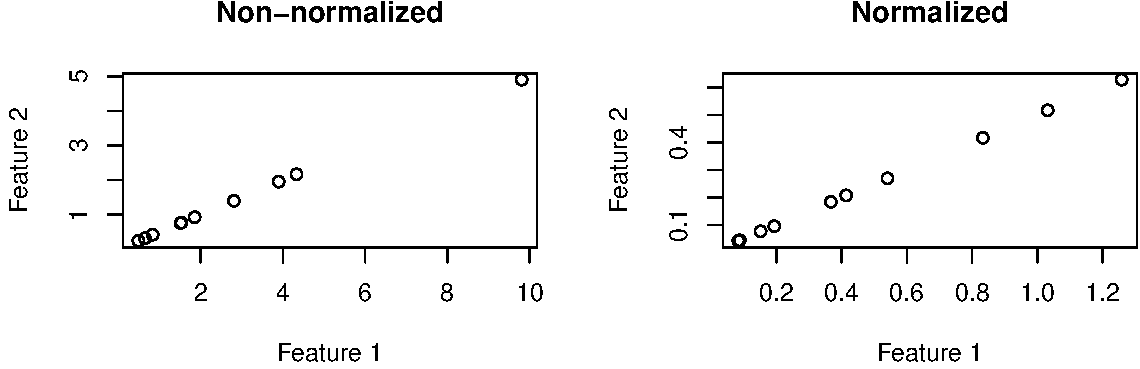
\includegraphics[width=\maxwidth]{figure/unnamed-chunk-16-1} \caption{Non-normalized and normalized associations between feature 1 and feature 2 of the second example.  Again, we expect to observe a positive association between feature 1 and feature 2.  In terms of generalized checkerboard scores, we would expect to see more co-variation patterns than co-exclusion patterns.  This is shown by the positive and relatively high value in the [1,2] element of test.output.  In this case, the smaller bin number yields a smaller NC-score because of the coarser partitioning of the data.}\label{fig:unnamed-chunk-16}
\end{figure}
\begin{kframe}\begin{alltt}
\hlstd{test.output}
\end{alltt}
\begin{verbatim}
##            Feature 1  Feature 2  Feature 3  Feature 4
## Feature 1  1.0000000  1.0000000  0.2000000 -0.3142857
## Feature 2  1.0000000  1.0000000  0.2000000 -0.3142857
## Feature 3  0.2000000  0.2000000  1.0000000 -0.2285714
## Feature 4 -0.3142857 -0.3142857 -0.2285714  1.0000000
\end{verbatim}
\end{kframe}
\end{knitrout}

\subsection{Example 3}

An example of using \Rfunction{nc.score} with user-defined bin edges.

\begin{knitrout}
\definecolor{shadecolor}{rgb}{0.941, 0.941, 0.941}\color{fgcolor}\begin{kframe}
\begin{alltt}
\hlstd{data} \hlkwb{<-} \hlkwd{matrix}\hlstd{(}\hlkwd{rlnorm}\hlstd{(}\hlnum{40}\hlstd{,}\hlkwc{meanlog}\hlstd{=}\hlnum{0}\hlstd{,}\hlkwc{sdlog}\hlstd{=}\hlnum{1}\hlstd{),}\hlkwc{nrow}\hlstd{=}\hlnum{10}\hlstd{,}\hlkwc{ncol}\hlstd{=}\hlnum{4}\hlstd{)}
\hlstd{data.rowsum} \hlkwb{<-} \hlkwd{apply}\hlstd{(data,}\hlnum{1}\hlstd{,sum)}
\hlstd{data[,}\hlnum{1}\hlstd{]} \hlkwb{=} \hlnum{2}\hlopt{*}\hlstd{data[,}\hlnum{2}\hlstd{]} \hlopt{+} \hlkwd{rnorm}\hlstd{(}\hlnum{10}\hlstd{,}\hlnum{0}\hlstd{,}\hlnum{0.01}\hlstd{)}
\hlstd{data.norm} \hlkwb{<-} \hlstd{data}\hlopt{/}\hlstd{data.rowsum}
\hlkwd{apply}\hlstd{(data.norm,}\hlnum{1}\hlstd{,sum)}  \hlcom{# The rows sum to 1, so the data are normalized}
\end{alltt}
\begin{verbatim}
##  [1] 1.1963684 1.1872435 0.5714268 1.2940662 0.2371974 0.7576704 1.0687281
##  [8] 1.9319371 1.3125265 0.6846835
\end{verbatim}
\begin{alltt}
\hlstd{test.input} \hlkwb{<-} \hlstd{data.norm}

\hlkwd{dimnames}\hlstd{(test.input)} \hlkwb{<-} \hlkwd{list}\hlstd{(}\hlkwd{paste}\hlstd{(}\hlstr{"Sample"}\hlstd{,}\hlkwd{seq}\hlstd{(}\hlnum{1}\hlstd{,}\hlnum{10}\hlstd{)),}\hlkwd{paste}\hlstd{(}\hlstr{"Feature"}\hlstd{,}\hlkwd{seq}\hlstd{(}\hlnum{1}\hlstd{,}\hlnum{4}\hlstd{)))}

\hlstd{test.output} \hlkwb{<-} \hlkwd{nc.score}\hlstd{(}\hlkwc{x}\hlstd{=test.input,}\hlkwc{bin.cutoffs}\hlstd{=}\hlkwd{c}\hlstd{(}\hlnum{0.1}\hlstd{,}\hlnum{0.2}\hlstd{,}\hlnum{0.3}\hlstd{))}
\end{alltt}
\end{kframe}
\end{knitrout}
\begin{knitrout}
\definecolor{shadecolor}{rgb}{0.941, 0.941, 0.941}\color{fgcolor}\begin{kframe}
\begin{alltt}
\hlkwd{par}\hlstd{(}\hlkwc{mfrow}\hlstd{=}\hlkwd{c}\hlstd{(}\hlnum{1}\hlstd{,} \hlnum{2}\hlstd{))}
\hlkwd{plot}\hlstd{(data[,}\hlnum{1}\hlstd{],data[,}\hlnum{2}\hlstd{],}\hlkwc{xlab}\hlstd{=}\hlstr{"Feature 1"}\hlstd{,}\hlkwc{ylab}\hlstd{=}\hlstr{"Feature 2"}\hlstd{,}\hlkwc{main}\hlstd{=}\hlstr{"Non-normalized"}\hlstd{)}
\hlkwd{plot}\hlstd{(data.norm[,}\hlnum{1}\hlstd{],data.norm[,}\hlnum{2}\hlstd{],}\hlkwc{xlab}\hlstd{=}\hlstr{"Feature 1"}\hlstd{,}\hlkwc{ylab}\hlstd{=}\hlstr{"Feature 2"}\hlstd{,}
     \hlkwc{main}\hlstd{=}\hlstr{"Normalized"}\hlstd{)}
\end{alltt}
\end{kframe}\begin{figure}[H]
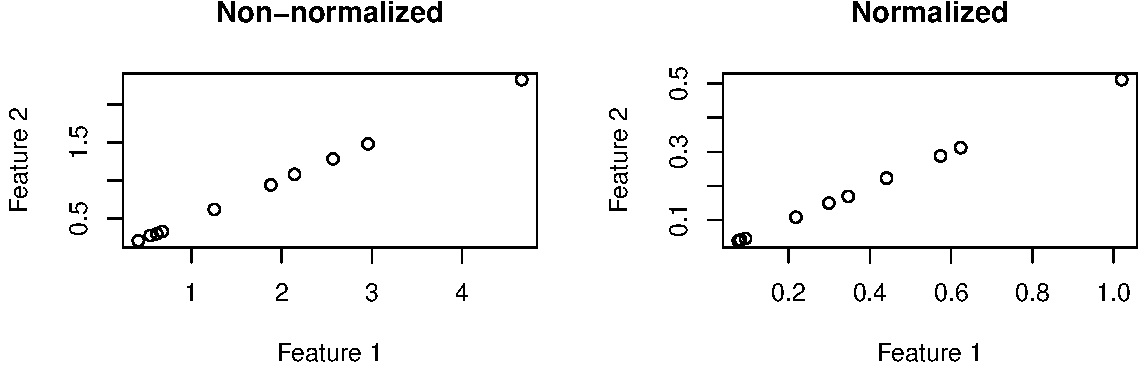
\includegraphics[width=\maxwidth]{figure/unnamed-chunk-18-1} \caption{Non-normalized and normalized associations between feature 1 and feature 2 of the second example.  Again, we expect to observe a positive association between feature 1 and feature 2.  In terms of generalized checkerboard scores, we would expect to see more co-variation patterns than co-exclusion patterns.  This is shown by the positive and relatively high value in the [1,2] element of test.output.  The bin edges specified here represent almost absent ([  0,0.001)), low abundance ([0.001,0.1)), medium abundance ([0.1,0.25)), and high abundance ([0.6,1)).}\label{fig:unnamed-chunk-18}
\end{figure}
\begin{kframe}\begin{alltt}
\hlstd{test.output}
\end{alltt}
\begin{verbatim}
##             Feature 1   Feature 2   Feature 3  Feature 4
## Feature 1  1.00000000  0.85628096 -0.08858079  0.4724309
## Feature 2  0.85628096  1.00000000 -0.02702703  0.2162162
## Feature 3 -0.08858079 -0.02702703  1.00000000 -0.4324324
## Feature 4  0.47243088  0.21621622 -0.43243243  1.0000000
\end{verbatim}
\end{kframe}
\end{knitrout}

%---------------------------------------------------------
\section{References} 
%---------------------------------------------------------

\bibliographystyle{plainnat}
\bibliography{ccrepe}

\end{document}
